%===============================================================================
% $Id: ifacconf.tex 19 2011-10-27 09:32:13Z jpuente $
% Template for IFAC meeting papers
% Copyright (c) 2007-2008 International Federation of Automatic Control
%===============================================================================
\documentclass{ifacconf}

\usepackage{graphicx}      % include this line if your document contains figures
\usepackage{natbib}        % required for bibliography
\usepackage{subfigure}
\usepackage{enumerate}
%===============================================================================
\begin{document}
\begin{frontmatter}

% Title, preferably not more than 10 words.

%Op��o 1 de titulo
%\title{DORIS: A MOBILE ROBOT FOR MONITORING OF OFFSHORE FACILITIES - THE EMBEDDED ELECTRONICS SYSTEM\thanksref{footnoteinfo}}

%Op��o 2 de titulo
\title{THE EMBEDDED ELECTRONICS AND SOFTWARE OF DORIS OFFSHORE ROBOT \thanksref{footnoteinfo}}

\thanks[footnoteinfo]{This work is supported primarily by Petrobras S.A. and
Statoil Brazil Oil \& Gas Ltda under contract COPPETEC 0050.0079406.12.9
(ANP-Brazil R\&D Program), and in part by the Brazilian research agencies CNPq
and FAPERJ.}

\author[1]{Renan S. Freitas}
\author[1]{Marco F. S. Xaud}
\author[1]{Ighor Marcovistz}
\author[1]{Alex F. Neves}
\author[1]{Rafael O. Faria}
\author[1]{Guilherme P. S. Carvalho}
\author[1]{Liu Hsu}
\author[1]{Eduardo V. L. Nunes}
\author[1]{Alessandro J. Peixoto}
\author[1]{Fernando Lizarralde}
\author[1]{Gustavo Freitas}
\author[1]{Ramon R. Costa}
\author[2]{P{\aa}l From}
\author[3]{Mauricio Galassi}
\author[4]{Peter W. J. Derks}
\author[5]{Anders R{\o}yr{\o}y}

%%% Op��o 1 de filia��o com email
%  \address[1]{Electrical
% Engineering Department, COPPE UFRJ, Rio de Janeiro, Brazil (renan028@poli.ufrj.br, marco.fernandes@poli.ufrj.br, imtz@poli.ufrj.br, alexfneves@poli.ufrj.br, rafael.o.faria@gmail.com, guilherme\_carvalho@poli.ufrj.br,\{liu,eduardo,jacoud,fernando,gfreitas,ramon\}@coep.ufrj.br, \{eduardo,sergioln\}@smt.ufrj.br)}
% \address[2]{Mathematical Sciences and Technology Department, Norwegian
%University of Life Sciences, Oslo, Norway (pafr@umb.no)}
% \address[3]{Research and Development Center, Petrobras/CENPES,
% Rio de Janeiro, Brazil (mauricio.galassi@petrobras.com.br)}
% \address[4]{TPD RDI Mature Area Development and Increased Oil recovery (MADI) , Statoil ASA, Bergen, Norway (aroy@statoil.com)}
% \address[5]{TPD RDI Frontier Developments (FD), Statoil Brasil \'{O}leo e G\'{a}s Ltda., Rio de Janeiro, Brazil (PEDE@statoil.com)}

%% Op��o 2 de filia��o sem email
  \address[1]{Electrical
 Engineering Department, COPPE UFRJ, Rio de Janeiro, Brazil}
 \address[2]{Mathematical Sciences and Technology Department, Norwegian
University of Life Sciences, Oslo, Norway}
 \address[3]{Research and Development Center, Petrobras/CENPES,
 Rio de Janeiro, Brazil}
 \address[4]{TPD RDI Frontier Developments (FD), Statoil Brasil \'{O}leo e G\'{a}s Ltda., Rio de Janeiro, Brazil}
 \address[5]{TPD RDI Mature Area Development and Increased Oil recovery (MADI) , Statoil ASA, Bergen, Norway}

\begin{abstract}                % Abstract of not more than 250 words.
DORIS is a research project which endeavors to design and implement a mobile
robot for remote supervision, diagnosis, and data acquisition on offshore
facilities. The proposed system is composed of a rail-guided robot capable of
carrying different sensors through the inspected area. This paper presents a
general overview of the robot, and a description of the developed embedded
electronics, power supply system and software architecture. Initial results
with teleoperated navigation validate the concepts considered so far and
rise several challenges for future works.
\end{abstract}

\begin{keyword}
mobile robots; field robotics; embedded electronics; power supply; robotic
software architecture;
\end{keyword}
%Guilherme: power supply como keyword? n seria melhor robotic power supply ou algo do tipo?

\end{frontmatter}
%===============================================================================

\section{Introduction}
The Oil \& Gas demand will grow rapidly in the next decades (\cite{wna}) and the
need to obtain the resources from hostile environments will increase operation
costs. Also, the working conditions on offshore installations, such as unfriendly atmosphere, heavy weather, extreme temperatures, constrained space, and the logistical issues are serious obstacles for Oil \& Gas companies. In order to be competitive, companies are looking into new and better technologies to be able to produce marginal fields and gain new resources. The use of robotics in inspection, maintenance, and repair operations in Oil \& Gas facilities could greatly improve efficiency, health and safety, while decreasing operational and logistics costs.

In the specific case of Brazil, the Oil \& Gas industry is growing at a high
pace. The recent discoveries of big oil fields in the pre-salt layer off the
Brazilian coast, located 300 km from the shore at depths of 5000 to 7000 km (\cite{presal}),
motivates the development of an offshore  production system with a high degree
of automation based on advanced robotics systems.

% It is highly expensive to have people working on the rig, as they
% must be housed and protected, there are costs with personal benefits such as
% health care, and the companies need to evacuate personnel quickly
% in case of an emergency.

Recent studies forecast a substantial decrease in the level of human operation
and an increase in automation on future oil fields (\cite{skourup2009robotized}).
The studies also point out the potential increase
in efficiency and productivity with robot operators, besides of the improvement in
Health, Safety, and Environment (HSE) conditions, as robots can replace humans
in tasks performed in unhealthy, hazardous, and confined areas (\cite{pal}).

\cite{chen} lists the challenges of robotics and automation in Oil
\& Gas industry:%and lists the most important requirements for robotic systems:

\begin{enumerate}[i)]
\item The \emph{atmospheric conditions} on offshore platforms are quite unfriendly, as
hydrocarbon resources can generate explosive and toxic gases;\\ %The robot should be certified to operate in explosive environments.
\item \emph{Corrosive agents}: splashy salty water, salty air and corrosive chemicals;\\
\item \emph{Weather}: high speed wind, squalls, rain and hail. The relative humidity is up to
100\% and ambient temperature can vary between $-30^{\circ}$C to $50^{\circ}$C. Possibly highly radiant heat from equipment and direct sunlight;\\
\item \emph{Constrained space} and/or walkways. Complex structures such as pipes,
flanges, tanks, and stairways.
\end{enumerate}

%There are different kinds of robots in the oil \& gas industry such as
%underwater pipeline repair robotic systems, robots for inspection of valve and
%lever position, gas level or leakage and acoustic anomalies monitoring, and
%robots for identify and locate fire.

Currently, the majority of the robotic systems in the Oil \& Gas industry are used for subsea tasks, such as mapping of the seabed, and inspection and repair of underwater equipment, risers and pipelines. However, recent research has focused on robotic applications on the topside of platforms to perform inspection and maintenance tasks, which includes valve and lever manipulation, gas level and leakage monitoring, acoustic anomalies diagnosis, and identification of smoke and fire.
%Guilherme: Senti falta de refs para a parte do subsea

The MIMROex inspection robot (\cite{mimroex}) was developed and
tested by the Fraunhofer Institute of Manufacturing Engineering and Automation
(IPA). The robot is capable of safely navigate in offshore environments, and
autonomously execute inspection tasks.

Sensabot (\cite{sensabot}), a teleoperated inspection robot developed by Carnegie Mellon University, was
designed for severe weather and atmosphere, being certified to operate in toxic, flammable and explosive environments.

%The robot includes the following sensors:
%\begin{enumerate}[i)]
%    \item Hydrocarbon sensor
%    \item Pan/tilt/zoom camera for remote operations
%    \item Temperature sensors
%    \item Vibration sensor for pumps, motors and bearings inspection
%    \item Microphone to detect audible machinery problems
%    \item Video camera to detect obstacles
%\end{enumerate}

The SINTEF Topside Robotic System, developed in the robotic lab facility in
Trondheim, Norway, is an intelligent instrumentation system designed to enable onshore operators
to monitor and control the platform's processes (\cite{kyrkjebo2009robotic}).

%In this paper, we describe the DORIS project, which aims to develop a mobile
%robot to perform monitoring and inspection in an
%offshore platform. To this end, the system must be able to move throughout the
%monitored environment carrying different sensors, analyzing sensor data
%\emph{in loco} or storing it for a posterior analysis, and interpreting the
%results. The sensors can identify abnormalities such as intruders in restricted
%areas, abandoned objects, smoke, fire, and liquid and gas leakages.
%Furthermore, the robot is able to make machinery diagnosis, read instruments,
%and takes samples using an embedded manipulator (\cite{cba}).

In this paper, we present a general overview of the DORIS robot, and a detailed description of the embedded electronics, power supply system and software architecture. The robot is designed to perform monitoring and inspection tasks in an
offshore platform, being able to move throughout the monitored environment carrying different sensors, analyzing sensor data \emph{in loco} or storing it for a posterior analysis, and interpreting the results. The sensors can identify abnormalities such as intruders in restricted areas, abandoned objects, smoke, fire, and liquid and gas leakages.
The robot is able to make machinery diagnosis, read instruments, and takes samples using an embedded manipulator (\cite{cba}).

This text is organized as follows: a general overview of the robot and its main
challenges are presented in Section \ref{sec:general_overview}, detailed
descriptions of the embedded electronics, the vehicle support system, power
supply system, and software architecture are taken in
Sections \ref{sec:electronics_overview}, \ref{sec:powersupply_overview}, and
\ref{sec:software} respectively.
In Section \ref{sec:results}, preliminary results are shown, and concluding
remarks are drawn in Section \ref{sec:conclusions}.

\section{General Overview}\label{sec:general_overview}

The DORIS robot contains a manipulator arm, cameras, microphones, and gas,
vibration and temperature sensors. The robotic device moves through a rail
and both of them are based on a modular concept.
Additional robot modules can be annexed to include extra sensors, and the rail
track can be modified by adding or replacing rail segments, thus enabling
operation in different areas of the platform. Figure~\ref{fig:DORIS-overview}
illustrates the operation in a production plant.

The robot is controlled autonomously or by teleoperation. Task managing
can be either in automatic (programmed using a mission interface) or manual
mode (real-time remote operation). The teleoperation and monitoring
capabilities guarantee online access to the embedded sensors, providing
information of the surrounding environment and the robot operating
conditions with real-time processing.


\begin{figure}[ht]
\centering
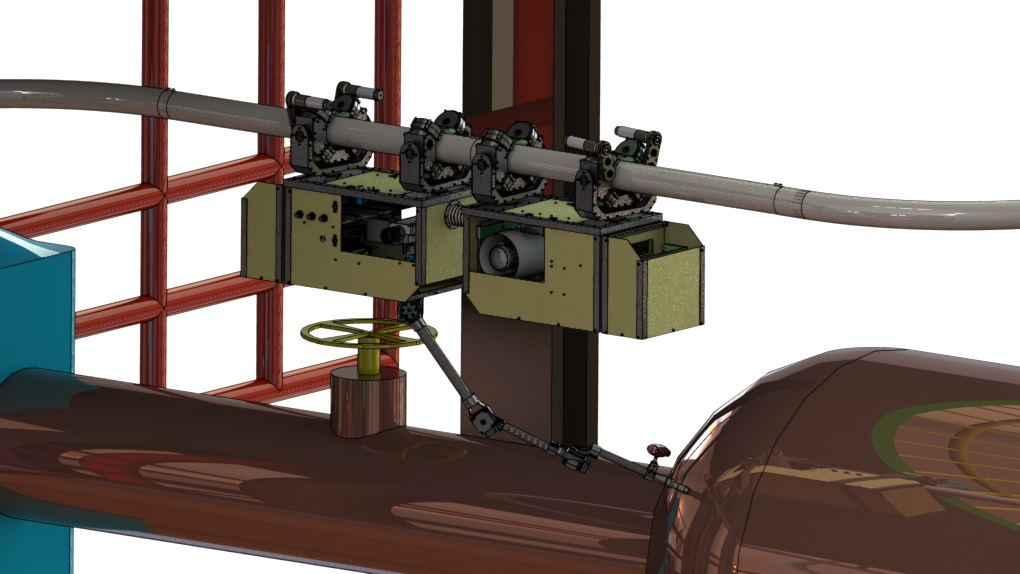
\includegraphics[width=8.4cm]{figs/cenario5.jpg}
\caption{Illustration of operation in a production plant.}
\label{fig:DORIS-overview}
\end{figure}

DORIS can be split into five subsystems: electronics, power
supply, software, mechanics and signal processing.

%-------------------------------------------------------------------------------------------------------------------------
%ELECTRONICS
%-------------------------------------------------------------------------------------------------------------------------
% The electronics subsystem is responsible for providing embedded computational
% support for the robot control, signal processing, task managing, and local and
% remote communication. The device motion is controlled through drivers that can
% receive position, velocity, or current setpoints. The embedded electronics has
% two printed circuit boards for the vehicle support system: energy distribution
% and monitoring, basic failure detection, emergency handling and devices'
% control.

%-------------------------------------------------------------------------------------------------------------------------
%POWER SUPPLY
%-------------------------------------------------------------------------------------------------------------------------
% The power supply system uses military-class lithium-ion batteries, which have
% small size and high energy capacity. In the first prototype of DORIS, four
% batteries are used to power the motors and two to power the other electronics
% components.


%-------------------------------------------------------------------------------------------------------------------------
%SOFTWARE
%-------------------------------------------------------------------------------------------------------------------------
% The main objective of the software subsystem is to allow the implementation of
% high- and low-level control of the robot. The tools used to develop DORIS
% software architecture must consider two important factors: they have to be
% commercially available, and provide modular functionalities. These requirements
% led to the adoption of Qt as the graphical interface framework ~\cite{qt},
% Robot Operating System (ROS) as the communication middleware ~\cite{ros}, and
% Ubuntu as the operating system.
%
% The software provides autonomous control (programmed tasks) and remote control
% through a Graphical User Interface (GUI) in the Host Control Base (HCB)
% computer. The HCB is composed of a set of processes running in parallel
% denominated ROS nodes, which can communicate with each other. To deal with this
% environment, a new software architecture called Robot Package Software is
% proposed, dividing the software into tools (graphical windows) and components
% (processing and communication unities), and grouping them into a dynamic
% library.

%-------------------------------------------------------------------------------------------------------------------------
%Mechanics
%-------------------------------------------------------------------------------------------------------------------------
The mechanics comprises the modules, the joints used to couple them, and the rail. The design allows the robot to move smoothly in a 3D space and to make a full stop anywhere on the track. It incorporates the use of gimbals with traction and guide wheels surrounding a tubular rail. The rail is designed to be as simple as possible, leaving the complexity to the robot, which is motivated by the fact that the rail may be extremely long so that the cost of it should be kept to a minimum. The use of two sets of gimbals provide mechanical compliance with rail curvatures, smoothness of the robot's base movement, and good weight distribution.

Considering the severe corrosion and weather conditions in offshore environments, the choice of materials is imperative for the success of the mechanical project and certified solutions must be considered if available.

The robot is composed of two modules in its default configuration, but it is conceived to be augmented with additional modules. The total weight of this basic configuration is estimated at 50 kg and DORIS can reach a maximum speed of 1m/s.

%-------------------------------------------------------------------------------------------------------------------------
%DSP
%-------------------------------------------------------------------------------------------------------------------------
The signal processing capabilities of the robot are:

\begin{enumerate}[i)]
  \item \emph{Video}: use
of multiple cameras (visible-light, infrared, panoramic, and stereo) to detect
video anomalies such as abandoned objects, smoke, fire, and liquid leakage;\\
  \item \emph{Audio}: detection of anomalies of impulsive nature, such as
an explosion, and machinery diagnosis based on energy and pitch
(fundamental frequency) signatures using a single or an array of microphones;\\
  \item \emph{Vibration analysis}: use of acceleration sensors to diagnose the operation mode
of rotating machines, performing possible fault classification, such as
 misalignment and unbalancing operation;\\
  \item \emph{Gas sensor}: detection of gas
 leakages;\\
  \item \emph{Mapping}: environment 3D model with a laser scanner.
\end{enumerate}

The main idea of all these signal processing features is to make the robot
perform an initial reference round on the closed rail track, being manually
validated by a system operator. In the subsequent rounds, all signal processing
algorithms compare the newly acquired signals with the reference data to detect
any form of anomaly, as indicated above. Once an anomalous behavior is
detected, an alarm is flagged to the system, which stores all associated data
for immediate or future diagnosis.
%round ou lap?

A detailed presentation of the mechanical and signal processing systems of DORIS can be found in \cite{OTC} and
\cite{cba}.

%-------------------------------------------------------------------------------------------------------------------------
%OTHER CHALLENGES
%-------------------------------------------------------------------------------------------------------------------------
Considering the robot functionalities and the aggressive offshore environment,
several challenges should be addressed. Regarding the robustness and safety required to operate in classified areas, the
robot must be: sealed against water and particles, resistant to a wide temperature
range, protected from impact and vibration, electrically shielded to avoid
explosion by ignition, and equipped with a monitoring system.

Another concern is that the embedded computers must run heavy signal
processing algorithms, requiring high computational power. However, the power
supply subsystem must efficiently provide power and maintain a low level of
power consumption.

Further complications arise because the system is designed to move in confined
areas and have efficient wireless communication with operators, providing
online information of sensors data.

%Temperatures in offshore facilities can
%vary between $-30^{\circ}$C to $50^{\circ}$C, relative humidity can reach
%100\%, and there may be splash water, salty air, storms, and high extensive
%corrosion ~\cite{graf2007mobile}.

\section{Embedded Electronics}\label{sec:electronics_overview}
The current embedded electronics (EE) is composed of a local central computer, a remote operation base and the following subsystems: communication, actuation, data acquisition, and an independent vehicle support system (VSS).

The \emph{computer} is the robot decision center, and it is in charge of: heavy data amount processing (video, images, audio and environmental data), data storing, data communication from/to other devices and the remote base, traction control and responding to other user commands. The computer is basically composed of a high performance Intel\textregistered Core\texttrademark i7 embedded in a PCIe/104 form factor board, RAM cards and SSD (\emph{solid-state drive}) card. This configuration permits the system easy expansion, and the SSD is a "no-moving part" solution that protects storage against vibration or other mechanical impact.

The remote operation base is the user workstation through where DORIS can be be remotely operated. This base can be located at any feasible site on the offshore facility. It is basically composed of a radio transceiver, a Wi-Fi access point and a computer system with a graphical user interface (GUI). The GUI includes buttons for DORIS control, buttons for device remote on/off, monitoring reports of current/voltage/temperature/failure, among other functions.

The \emph{communication system} is in charge of the data traffic within the robot and between the robot and the remote base. This system is composed of:

\begin{enumerate}[i)]
  \item \emph{Local Gigabit Ethernet} network: for heavy data real-time traffic within the robot, such as video, audio and commands from/to the computers;\\
  \item \emph{Controller Area Network} (CAN) bus for communication of control commands to the actuation system;\\
  \item \emph{Wireless technologies} between the robot and the remote operation base: DORIS can be remotely operated from this base via Wi-Fi IEEE 802.11n or via 2.4/5.0 GHz radio links (upon Wi-Fi absence or failure). There are two Wi-Fi access points: one placed on the robot and another one at the remote base (also, one radio transceiver on the robot and another on the base).
\end{enumerate}

The Ethernet network has a star topology centralized by an OSI-Layer 2 Switch,
and connects the computer, Ethernet peripheral devices (such as cameras), a local Wi-Fi access point and the vehicle support system (VSS). This network topology allows easy expansion of the Ethernet network for additional wagons. Together, the Ethernet network and Wi-Fi form a \emph{Local Area Network} (LAN).

DORIS traction is taken by the \emph{actuation system}, which is composed of four controller drivers (Maxon Motor EPOS2 70/10), and four motor packs, each containing a high power 200 W EC-4pole Maxon Motor brushless motor, an encoder and a planetary gearhead (with 21:1 reduction rate).

The \emph{actuation system} is commanded by the computer via CAN bus, which
provides reliability, safe transmission and the appropriate speed to this
application (\cite{can}). The interface between the computer and the CAN bus is a dual channel board compatible with PCI-express bus, which is present at the PCIe/104 computer module board. Since the traction system generates a significant amount of conductive noise, a galvanic opto-isolator is embedded in the CAN interface to minimize interference on the rest of the EE system.

% Gustavo: Falar do Watchdog do alex.
% Guilherme: Nao sera falado agora

The current \emph{data acquisition system} is in charge of the acquisition of images, video, audio from the environment. It is composed of a fixed camera, an infrared thermal camera (which gives both a thermal map and temperature measurement), a \emph{fisheye} camera, and two stereoscopic webcams (with embedded microphone). All cameras have Ethernet interface, except the webcams (USB).

An overall scheme of DORIS EE system is shown in Fig.~\ref{fig:EE-Communications}.

\begin{figure}
\begin{center}
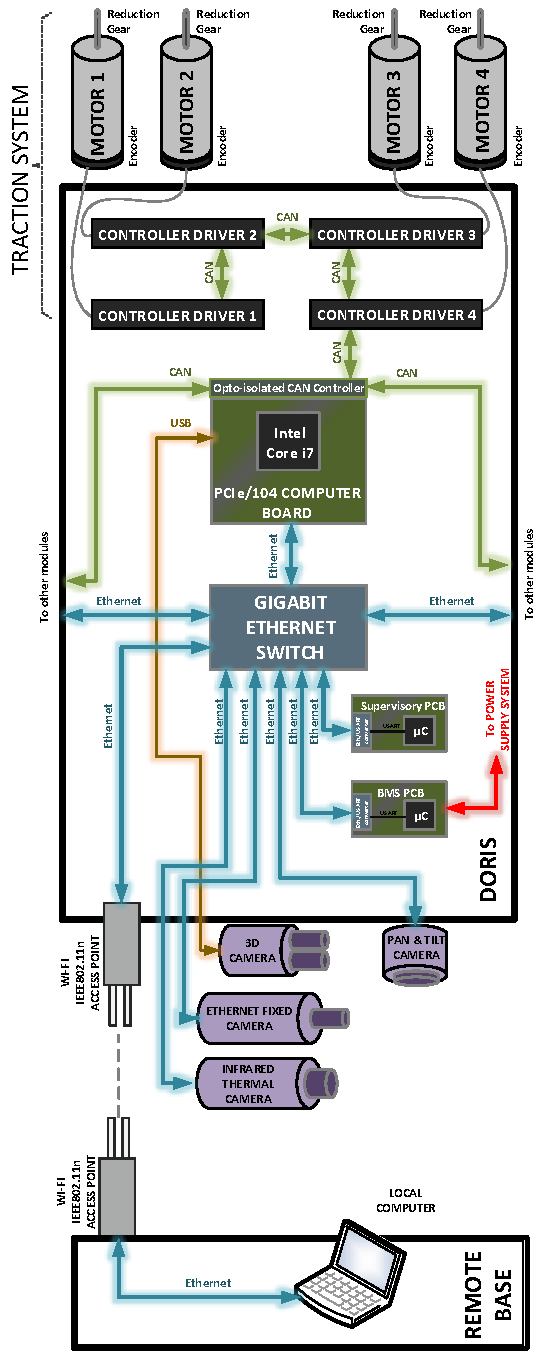
\includegraphics[width=8.4cm]{figs/EE-Communications.pdf}
\caption{Overall scheme of DORIS EE system.}
\label{fig:EE-Communications}
\end{center}
\end{figure}

\subsection{Vehicle Support System}\label{sec:VSS}

The \emph{Vehicle Support System (VSS)} (\cite{MARIUS}) is composed of
microcontroller based \emph{printed circuit boards} (PCBs) designed for:

\begin{enumerate}[i)]
    \item \emph{Failure detection}, achieved by the monitoring of devices'
    current/voltage and module internal temperature/humidity;\\
    \item \emph{Device protection} against overcurrent by fuses and
    solid-state relays, which can be turned on/off at any time automatically,
    upon a detected failure, or manually via operator;\\
    \item \emph{Energy distribution and monitoring}, achieved by the \emph{Battery
    Management System (BMS)}. Each battery pack is monitored via \emph{System Management Bus} (SMBUS)
    communication, which allows the reading of the battery status, voltage,
    current, temperature, remaining charge, and other variables. This
    information allows the VSS to provide adequate power balance in extreme situations (e.g.: demand of full power to
    either the traction system or the electronics system) or reconfiguration of
    power supply distribution in case of failures;\\
    \item \emph{Emergency handling}: the robot can be turned on/off using a physical
    \emph{emergency shutdown (ESD)} button or via radio. The radio system can
    also replace Wi-Fi in some functionalities if it fails or are simply unavailable.
  \end{enumerate}

DORIS VSS includes three types of PCBs: supervisory, BMS and power bus switching.

The \emph{supervisory PCB} is basically composed of ATMEL AVR AT90CAN64 microcontrollers, solid-state relays (max. 1.5 A), hall effect sensors,
16-channel analog-to-digital converter (ADC), an I$^{2}$C temperature/humidity (T/H) sensor, and an Ethernet-to-UART converter. It is in charge of monitoring and protecting the robot devices. The monitoring functions collects the module supply voltages using the AVR embedded ADC, the module temperature and humidity using the T/H sensor,
and the devices' supply currents using hall sensors and an external 16-channel ADC for data interpretation.

The AVR microcontrollers manage the collected data, report it periodically to DORIS computer via Ethernet, and locally detect or react to faulty situations. Since Ethernet is not an available interface in this AVR
model, an UART-to-Ethernet converter is used for data communication. The local fault
detection is done by pre-programmed algorithms in the microcontroller, which reacts
to protect devices against overcurrent. This is done by commanding
the open/close state of the relays, hence turning off the devices. All these AVR
functionalities can also be commanded by the remote operator.

The \emph{BMS PCB} is in charge of managing the power supply system. It communicates with the batteries via SMBUS and has a connection with the power bus switching PCB. SMBUS is the interface of the telemetry system embedded in DORIS battery model. This system collects important information from the batteries, such as temperature, voltage, current and remaining charge.
% Zeka: Verificar se � mesmo enrola��o

The \emph{power bus switching PCB} contains high power solid-state relays (20 A), which
can be commanded from the BMS PCB to distribute the power of each battery pack to
either motor bus or electronics bus. The decisions about the better
power balancing are based primarily on data collected via SMBUS.

\section{Power supply system}\label{sec:powersupply_overview}
The power supply system is responsible for the safe, reliable, and
efficient electric power distribution for DORIS devices. The power is supplied by
high density energy level military lithium ion battery technology, which comes
with an intrinsically safety circuit for protection against short-circuits and
heating. Each battery pack support has a capacity of 10 Ah at 24V. According to
mechanical constraints, each DORIS module admits a maximum of four battery
packs, each one weighing 1.4 kg.
% Zeka: Verificar compara��o de baterias se vale ou nao a pena
% Ighor: Acha encher lingui�a demais.

As \cite{verma2004real} highlights, field robots often
operate in environments where human intervention is expensive, slow,
unreliable, or impossible. Therefore, it is essential to monitor their behavior
so that faults may be addressed before they result in dangerous failures. For
proper power management, the electronics system uses information about each
battery condition, such as battery voltage, current, temperature and remaining
charge. The BMS PCBs read the batteries data via SMBUS protocol, as described in section \ref{sec:VSS}.

In order to avoid electromagnetic (EMI) and conductive noise interference
caused by the robot motors, the system currently works with two separate power
buses, each one using two 24 Vdc batteries connected in parallel,
being able to deliver 20 Ah. One bus is dedicated to power the
motors and the other to all electronic devices.

DC/DC converters are employed to create different voltage levels (12 Vdc and 5 Vdc) and
ensure a stable power source, even for 24 Vdc components. To achieve power protection, diodes are used to avoid back-flow
current, fuses protect the system from undesired peaks, and buttons allow power
buses to be separately turned on/off.

The electronics power bus uses 14 AWG wires for up to 15 A of nominal current and the motors power bus uses 12 AWG wires for up to 21 A of nominal current. The power supply architecture is illustrated in Fig.~\ref{fig:DiagramaSAM}.

Since DC batteries are the power source of the robot, there is no need of a capacitor to correct delays between current and voltage. However, a capacitor bank would allow additional energy to the motors.

If the source energy is a battery, then the capacitor bank must have at least 400 to 500 $\mu F$ for each
Ampere (\cite{capacitor}). In the case of DORIS, as each motor may require a peak current
of 20 A, a capacitor bank dedicated for each driver would need between 8000 and
10000 $\mu F$, and the use of small capacitors in parallel would be an option.

It is also recommended to have the maximum operating voltage of the capacitor
bank at around 50\%, ie, 35 V since the battery voltage is 24 V. In
this case, one must use electrolytic capacitors, as other types of
capacitors are not able to provide this capacitance value at this voltage level.
The capacitor should have low equivalent series resistance and should be located as
close as possible to the noise source, namely the motors.

\begin{figure}[ht]
\centering
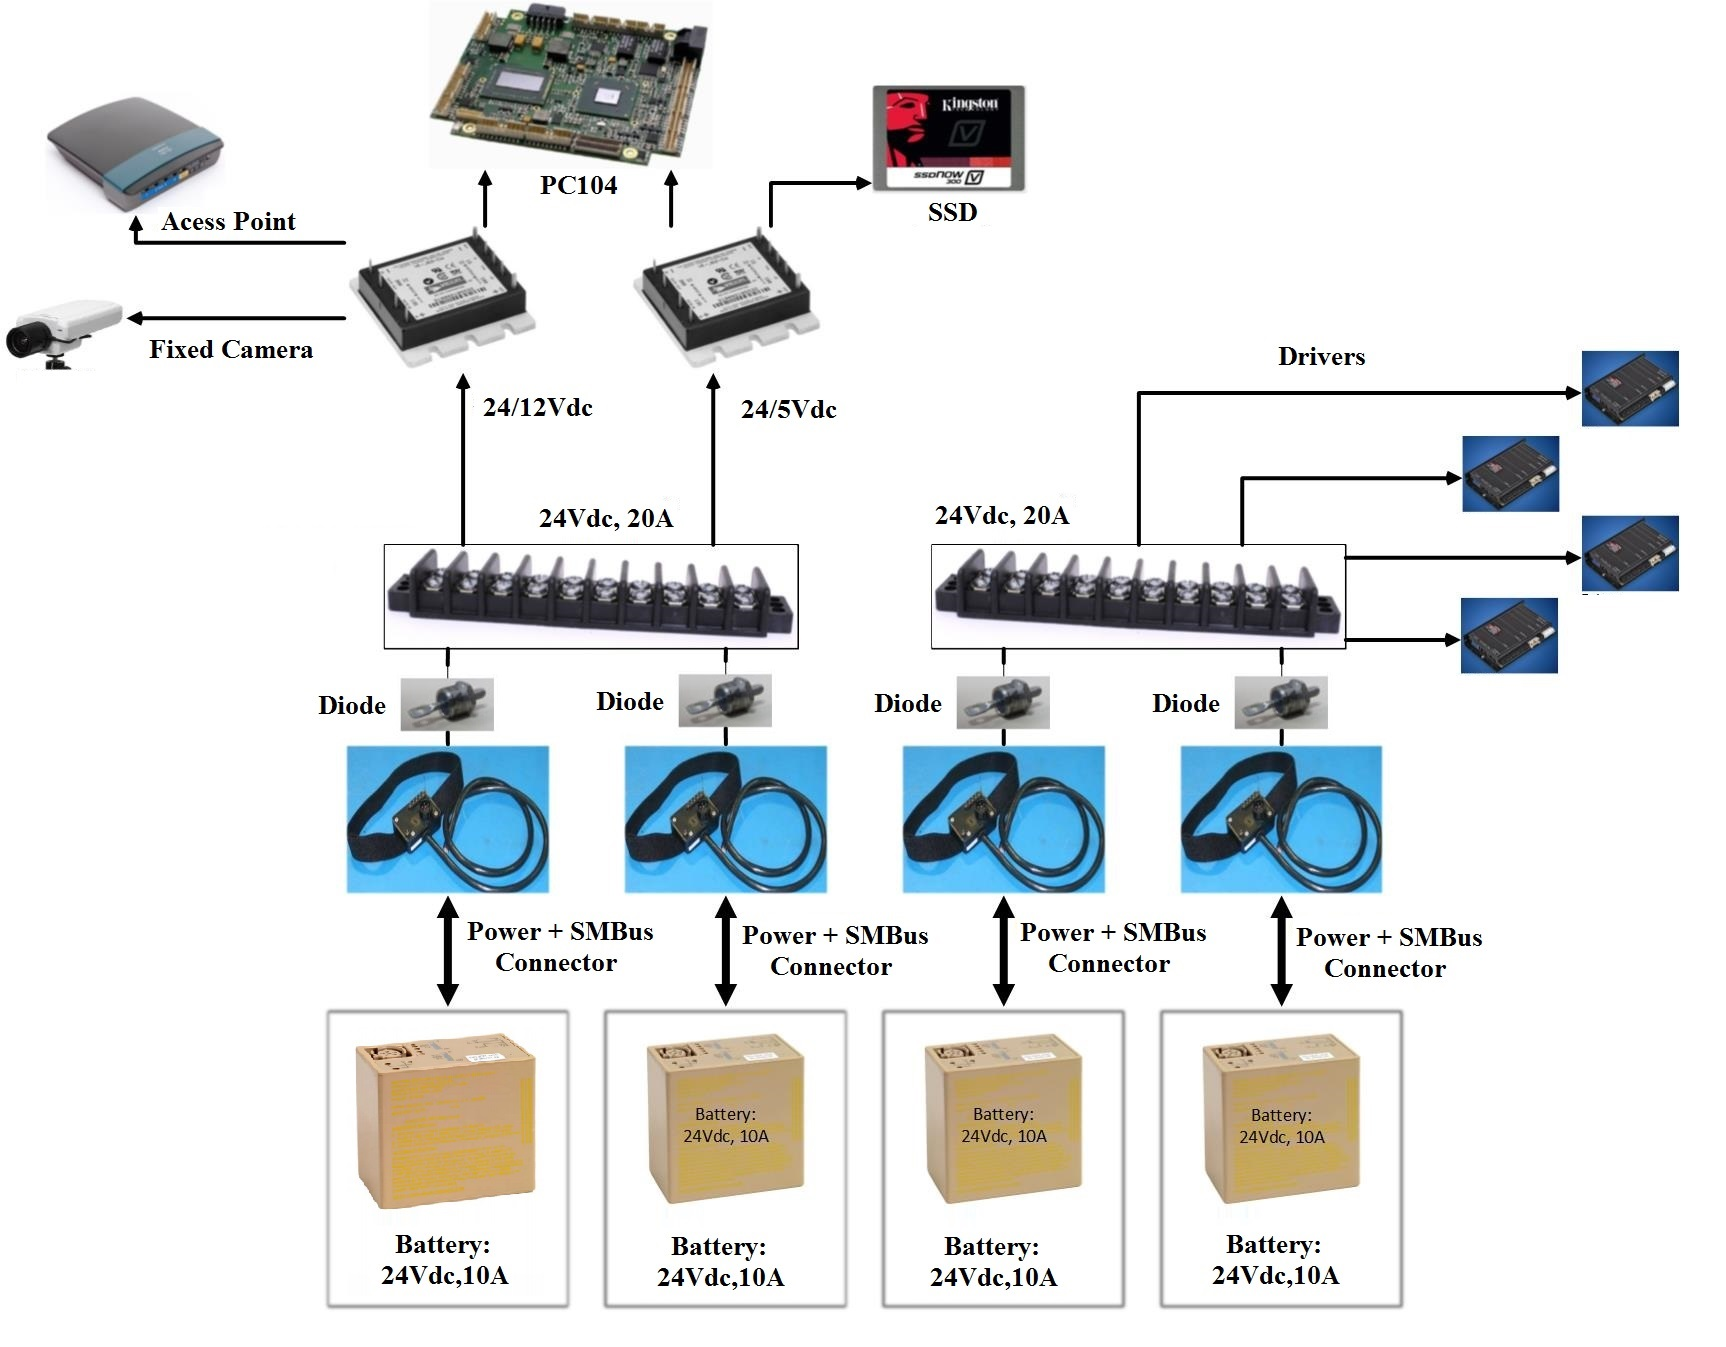
\includegraphics[width=1\columnwidth]{figs/DiagramaSAM.jpg}
\caption{DORIS power supply architecture.}
 \label{fig:DiagramaSAM}
\end{figure}

%Considering this, new challenges arise in order to improve the features of
%the system.
%Gustavo: Frase muito largada!

\section{Software System}\label{sec:software}

The software subsystem allows the implementation of high and low level control
of the robot. The DORIS software architecture considers two important factors:
all tools have to be open-source, and they have to provide modular
functionalities.
These requirements led to the adoption of Qt as the graphical interface
framework (\cite{qt}), Robot Operating System (ROS) as the communication
middleware (\cite{ros}), and Linux/Ubuntu as the operating system.


The software provides autonomous control (programmed tasks) and remote control
through a Graphical User Interface (GUI) in the Host Control Base (HCB)
computer. In both computers (robot and HCB), a set of processes, denominated \emph{ROS
nodes}, runs in parallel and can communicate with each other.

To deal with this specification, a software framework, named \emph{Robot Package Software} is proposed, which is based on tools (graphical windows) and components (processing and communication unities) grouped into a
dynamic library, \emph{libRobotPackage.so}. The Robot Package is a general package
which can be used for another robotic systems. Additionally, a more specific
package, \emph{DORIS package}, is proposed to deal with DORIS hardware and
functionalities. It is a library (\emph{libDORISPackage.so}) containing a
list of components and tools for the DORIS robot.

A robot 3D model based on ROS \emph{Unified Robot Description Format} (URDF),
which is an XML format to represent a robot model, is presented in Fig.~\ref{fig:rviz}.
The 3D model, which includes the rail and the robot system, is integrated in the GUI and can be
visualized using RVIZ (a ROS tool). Thus, the robot motion can be visualized
in the GUI and the operator can control the robot in the 3D environment by
marking a desired setpoint position on the interface.

\begin{figure}[!h]
\centering
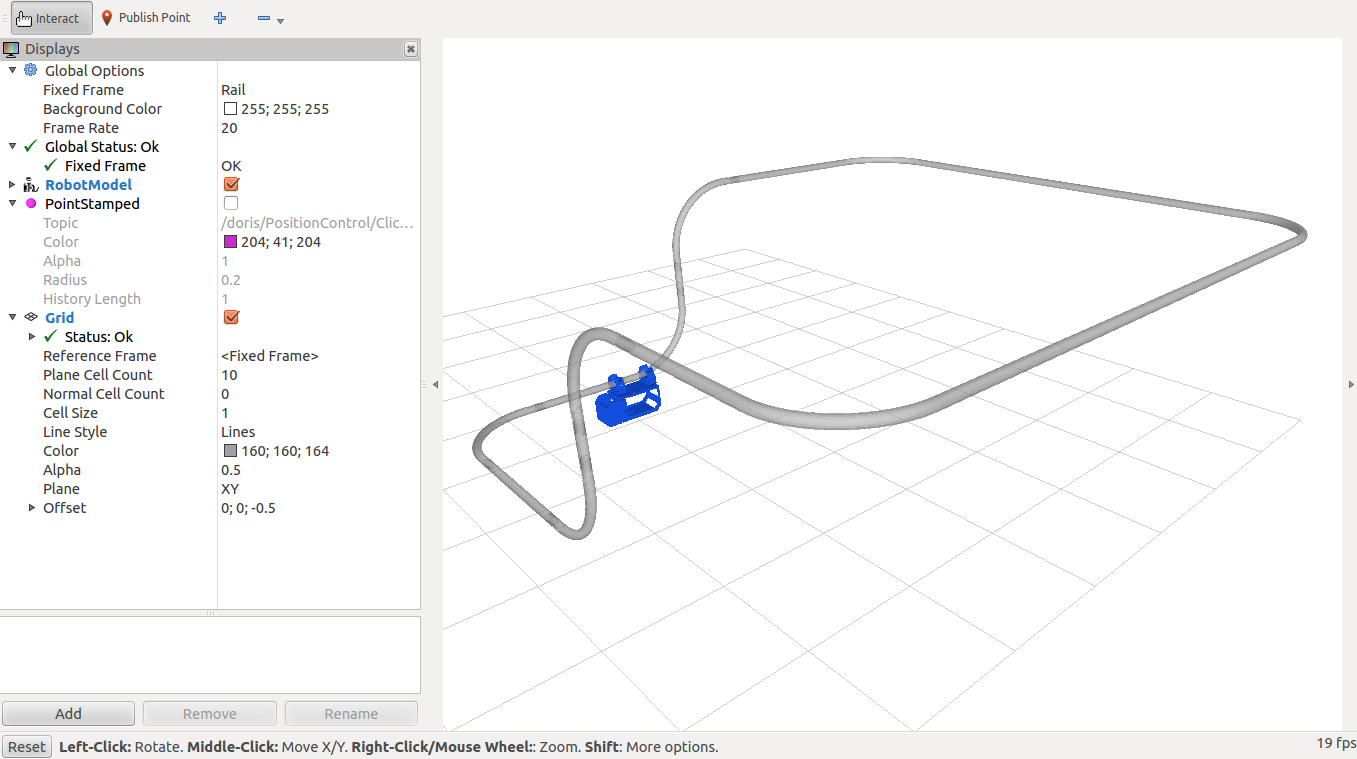
\includegraphics[width=8.4cm]{figs/rviz.png}
\caption{Robot system 3D model.}
\label{fig:rviz}
\end{figure}

A Web tool is also proposed to remotely control DORIS using a standard internet
browser with \emph{javascript} support (Fig.~\ref{fig:teleop}). The webtool is based
on \emph{rosbridge} and \emph{javascript} libraries \emph{roslibjs}, \emph{ros2js} and \emph{ros3djs}.

\begin{figure}[!h]
\centering
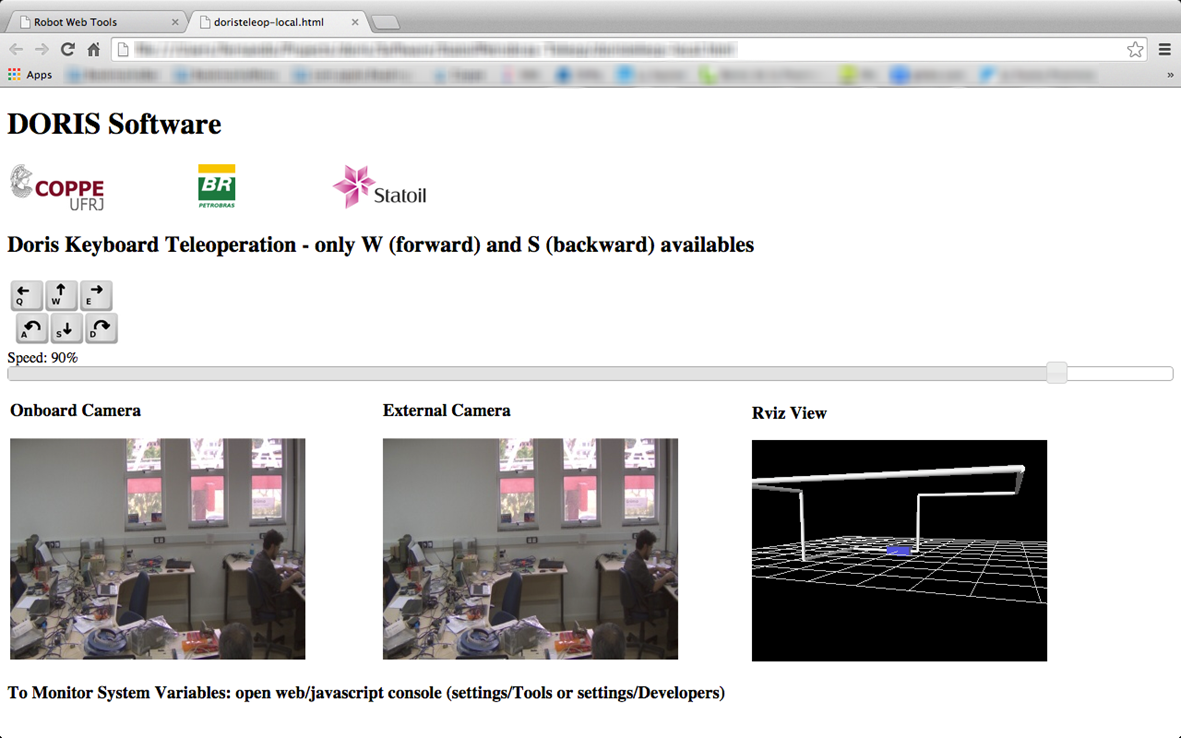
\includegraphics[width=8.4cm]{figs/teleop.png}
\caption{Web tool to remotely control DORIS using a standard internet browser.}
\label{fig:teleop}
\end{figure}
%Gustavo: trocar imagem!


\section{Experimental tests and results}\label{sec:results}
A prototype named \emph{Single Autonomous Module} (SAM) was built to verify the previous proposed concepts. In addition, some VSS functionalities were individually tested, but not yet fully integrated with SAM. The subsections \ref{sec:SAM_tests} and \ref{sec:VSS_tests} below detail the executed tests.

\subsection{Single Autonomous Module (SAM)}\label{sec:SAM_tests}
SAM (Fig.~\ref{fig:SAM2}) is a single module composed of an AXIS ethernet fixed
camera, two USB Minoru stereoscopic Webcams, a Cisco wireless router, four EC-4pole 200 W motors and
Maxon EPOS2 drivers, a PCIe/104 with Intel Core i7 computer module, 4GB DDR3 RAM, 240GB SSD (Kingston), a dual-channel opto-isolated PCI-express CAN interface, and few PCBs.

SAM was tested in horizontal and vertical motion on a closed rail made of straight and curved PVC tubes. The curved segments are straight tubes of 1 m bent by $90^{\circ}$, resulting in a curvature of approximately 630 mm. The complete track has 23 m length and comprises all the possible robot motion types. The rail was installed in the
GSCAR laboratory, in COPPE/UFRJ (Brazil), and SAM was able to fully move throughout the entire track.

Concerning electronics, power supply, and software, the first objectives of SAM were to test the following concepts:
\begin{enumerate}[i)]
  \item \emph{Electronics}: sensor integration and communication system;\\
  \item \emph{Power supply}: independent buses for motors and electronics devices, and batteries robustness and duration;\\
  \item \emph{Software}: teleoperation and user interface.
  \end{enumerate}

\begin{figure}[!h]
\centering
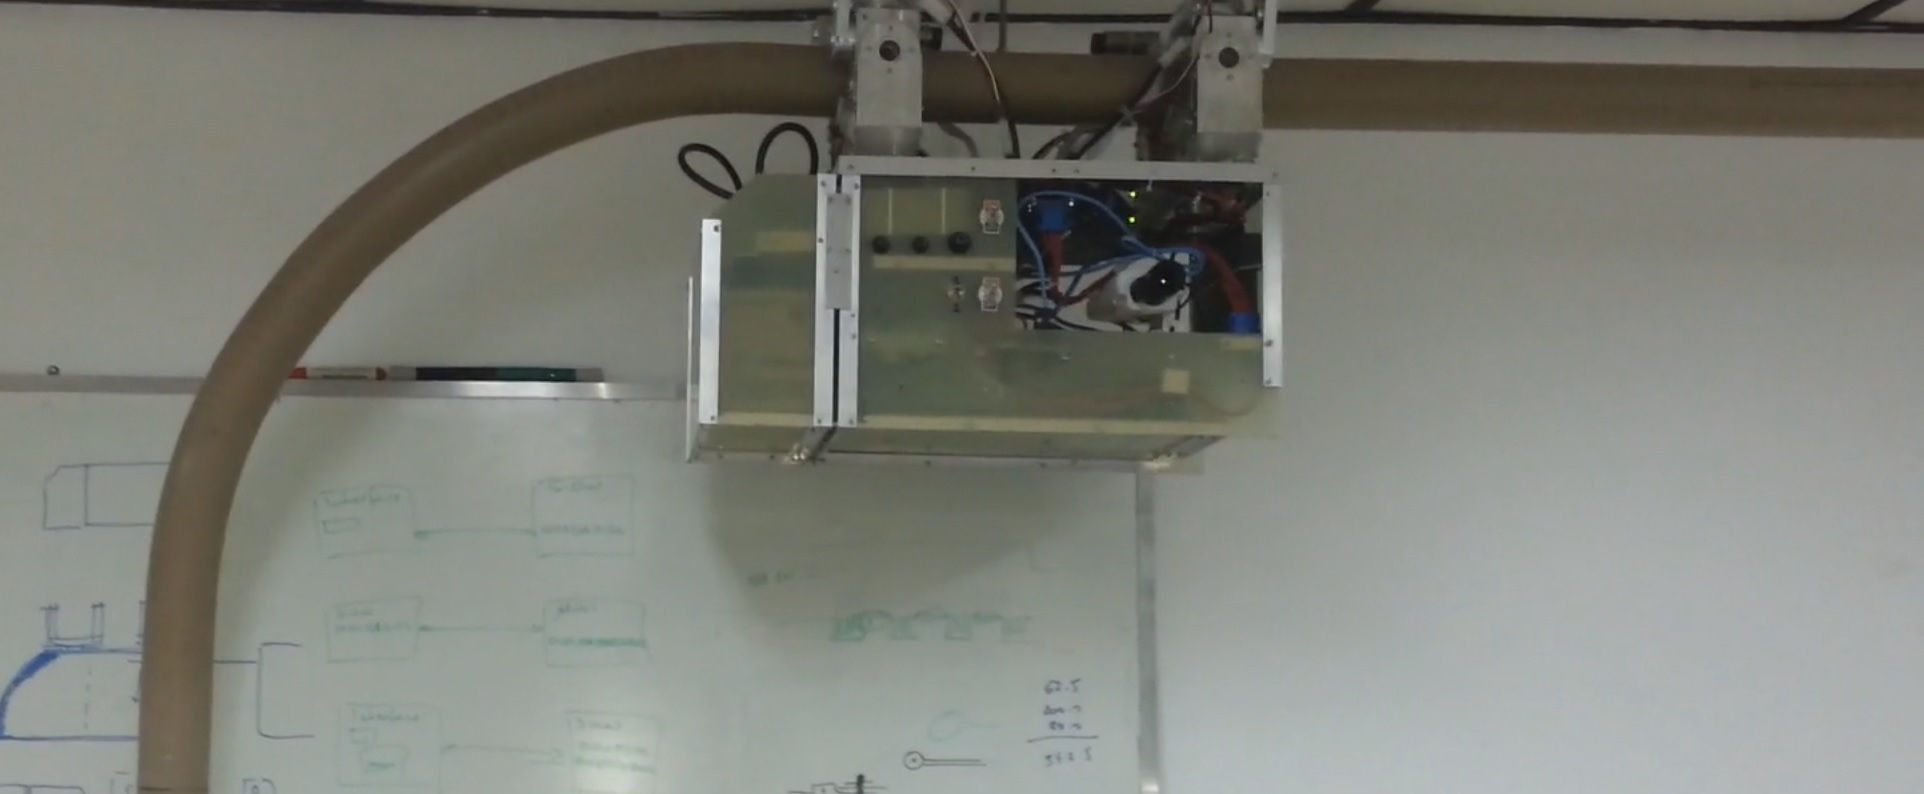
\includegraphics[width=8.4cm]{figs/SAM4.jpg}
\caption{SAM - Single Autonomous Module.}
\label{fig:SAM2}
\end{figure}

The communication system was implemented: \emph{Ethernet communication network}
to connect the fixed camera, the computer, and the access point; \emph{Wi-Fi
communication network} to connect SAM with the base; \emph{CAN bus} to
control the actuation system; and two stereoscopic Webcams were plugged to the
computer through USB connections. As Wi-Fi 
All the communication networks worked properly, as
expected.

The concept of independent power buses proved to be efficient, and the designed
battery capacity could handle the system energy demand. However, it was
observed that when SAM moves downwards, the motors brake the robot instead of accelerating it,
and generate a brake energy on the way back to the source.
Depending on the length of the downhill section and the robot's speed, this energy may reach a
voltage level that causes the motors drivers to reset. This issue must
be further studied to investigate if it is worth to store
this extra energy or simply waste it using an additional device to dissipate this energy as heat.

Furthermore, it was verified that SAM can be teleoperated from anywhere by
accessing its Wi-Fi network and the GUI (\emph{Graphical User Interface})
developed in Qt environment. SAM has already been teleoperated by Petrobras
(from Brazil) and by Statoil (from Norway).

\subsection{Vehicle Support System (VSS) Tests}\label{sec:VSS_tests}
All DORIS VSS functions were successfully tested independently. The AVR firmware was programmed in C++ using Atmel Studio 6.1.
The following tests/implementations were successfully performed:
\begin{enumerate}[i)]
    \item Logic to command the \emph{solid-state relays} to turn on/off some devices: the
    relays can be opened/closed via RS485 commands from the notebook;\\

    \item Acquisition of \emph{module voltages}: DC-DC voltage (5, 12 and 24 VDC) and battery raw voltage measurements can be accessed via RS485 commands from the notebook. The voltage is measured using the AVR embedded ADC;\\

    \item Acquisition of \emph{module currents}: the measurement of the currents that
    supply each device can be read via RS485 commands from the notebook. The
    currents are sensed using hall-effect sensors. The microcontroller embedded
    ADC doesn't have enough measuring ports, thus an external one is
    used to digitalize the current measurements;\\

    \item Acquisition of \emph{module temperature/humidity}: the measurements of
    the module temperature and humidity can be read via RS485 commands from the
    notebook. A specific T/H sensor is used for this acquisition;\\

    \item Acquisition of \emph{battery information}: voltage, temperature,
    current, remaining charge, and battery status can be read via RS485 commands
    from the notebook. The acquisition of all battery data is implemented using
    SMBUS communication;\\

    \item \emph{Timers} to enable robot shutdown in predetermined time and periodic data report of voltages, currents, relays status, temperature, and humidity.
\end{enumerate}

\section{Conclusion and Future work}\label{sec:conclusions}

In this paper, we presented the embedded electronics and software subsystems of the DORIS
project, which endeavors to develop an offshore facilities inspection and monitoring robot.

%The prototype is based on rail guided modules powered by a battery system and equipped with multiple
%sensors that enable the detection of anomalies, such as abandoned objects and
%gas leakage.

A prototype, SAM, was built to test electronics, power supply, and software architecture concepts.
Preliminary results show good overall performance of sensor integration and communication, independent power buses for electronics and motors, and teleoperation.

The Vehicle Support System was tested outside the robot and the customized printed circuit boards were able to monitor the batteries via SMBUS, temperature and humidity, DC/DC voltage levels, and the devices' currents.

%The solid-state relays can also turn on/off the devices for protection and/or
%efficiently power consumption.

Ongoing implementations and future challenges include:
\begin{enumerate}[i)]

  \item \emph{New VSS tests}:\\
  RS485 will be replaced by UART to allow communication with the PCs via Ethernet network, the control of BMS high-power relays will be implemented in AVR to allow the management of DORIS energy power distribution, and the logic that uses the SMBUS data to manage DORIS energy distribution will be applied;\\

  \item \emph{Expansion and reconfiguration of robot modules}:\\
  DORIS will need more than one module to support all the defined devices and features.
  The EE system permits the free expansion and reconfiguration of DORIS modules, enabled by the bus topology for DORIS main networks: Ethernet and CAN.\\

  \item \emph{Autonomous operation}:\\
  DORIS autonomous operation is a challenge for the software development. The
  Positioning System, which currently comprises wheels' encoders (odometry) and a
  fixed camera (3D mapping), will be upgraded with an inertial movement unit
  (IMU) and the detection of rail landmarks, such as rail supports and segments connections. The fusion of these measurements will help to estimate the vehicle states, such as position, attitude and velocity;\\

  %Novo item sobre mission control?
  %Also, a Mission Control System need to be developed for the operator.\\

  \item \emph{Reduced interferences, such as EMI and electrostatic charge}:\\
  Future improvements should include a well design and installation of the
  shield network and grounding system to reduce EMI. An electrostatic discharger
  should be designed to drain the accumulated charge from the shielding system;\\

  \item \emph{Solution for DORIS downhill motion issue:}\\
  The regeneration issue imposes overvoltage on the drivers, which may reset
  during the downhill motion. To prevent it, a shunt regulator
  will be used to dispose the extra energy and avoid the overvoltage issue.
  It represents a solution, but wastes this energy, while a
  big capacitor bank could be used as an energy storage device. Tests will be held to measure the
  generated amount of energy to decide if it is worth to embed a device to store or waste it;\\

  \item \emph{Hardware Certification:}\\
  The robot must be certified to operate in corrosive environments and explosive atmospheres.
\end{enumerate}

\bibliography{ifacconf}

\appendix

\end{document}
